\documentclass{article}
\usepackage{tikz} 
\usepackage[utf8]{inputenc}
\usepackage{amsmath}
\usepackage{listings}
\usepackage{amsfonts}
\usepackage{amssymb}
\usepackage{tabularx}
\usepackage{enumitem}
\usepackage{algorithm}% http://ctan.org/pkg/algorithm
\usepackage[noend]{algpseudocode}% http://ctan.org/pkg/algorithmicx
\usepackage{tikz}
\usepackage{graphicx}


\usepackage{subcaption}
\usepackage{multicol,caption}
\usepackage{geometry}
 \geometry{
 a4paper,
 total={210mm,297mm},
 left=20mm,
 right=20mm,
 top=20mm,
 bottom=20mm,
 }

\usetikzlibrary{arrows,positioning,shapes,fit} 
\pgfarrowsdeclarecombine{ring}{ring}{}{}{o}{o}
\thispagestyle{empty}
\DeclareMathOperator{\ringarrow}{\raisebox{0.5ex}{\tikz[baseline]{\draw[ring->](0,0)--(2em,0);}}}

\definecolor{talk}{HTML}{729FCF}
\definecolor{talk2}{HTML}{E8A753}
\definecolor{grey}{HTML}{DBDCDD}
\renewcommand{\vec}[1]{\boldsymbol{#1}}
\tikzset{
    %Define standard arrow tip
    >=stealth',
    %Define style for boxes
    observed/.style={
   	circle,
   	rounded corners,
   	draw=black, thick,
   	minimum width=2.3em,
   	minimum height=2.3em,
   	font=\footnotesize,
   	text centered,
   	fill=talk!50
   },
   latent/.style={
   	circle,
   	rounded corners,
   	draw=black, thick, dashed,
   	minimum width=2.2em,
   	minimum height=2.2em,
   	font=\footnotesize,
   	text centered
   },
    % Define arrow style
    pil/.style={
           o->,
           thick,
           shorten <=2pt,
           shorten >=2pt,},
    sh/.style={ shade, shading=axis, left color=red, right color=green,
    shading angle=45 },
observedrect/.style={
	rectangle,
	rounded corners,
	draw=black, thick,
	minimum width=3em,
	minimum height=1.5em,
	font=\footnotesize,
	text centered,
	fill=talk2!80
},  
 target/.style={
	circle,
	rounded corners,
	draw=black, thick,
	minimum width=2.3em,
	minimum height=2.3em,
	font=\footnotesize,
	text centered,
	fill=talk2!80
},
empty/.style={
	circle,
	rounded corners,
	minimum width=.5em,
	minimum height=.5em,
	font=\footnotesize,
	text centered,
},
}
   
\begin{document}
\pagestyle{empty}

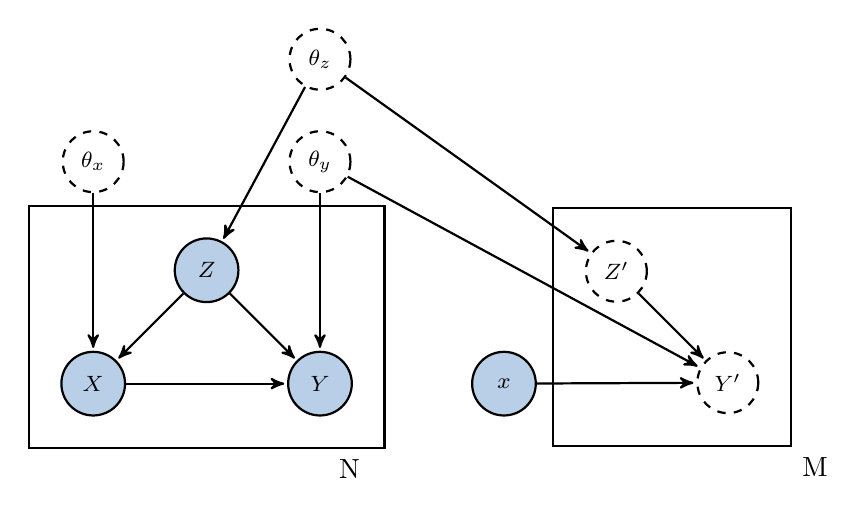
\begin{tikzpicture}[->,>=stealth',shorten >=1pt,auto,node distance=1.2cm, thick,node/.style={observed},lt/.style={latent}]
\tikzstyle{box}=[rectangle, draw=black!100]
%nodes
\node[node](1){$Z$};
\node[node, below left=of 1](2){$X$};
\node[node, below right=of 1](3){$Y$};
\node[node, right=1.5cm of 3](4){$x$};
\node[lt, above right=of 4](5){$Z'$};
\node[lt, below right=of 5](6){$Y'$};
\node[lt, above=2.0cm of 3](9){$\theta_{y}$};
\node[lt, above=0.5cm of 9](7){$\theta_z$};
\node[lt, above=2.0cm of 2](8){$\theta_x$};
\path[every node/.style={font=\sffamily\small}]
(1) edge (2) edge (3)
(2) edge (3)
(4) edge (6)
(5) edge (6)
(8) edge (2)
(7) edge (1) edge (5)
(9) edge (3) edge (6);
\node[rectangle, inner sep=4.0mm, fit= (1) (2) (3),draw=black!100,label=below right:N] {};
\node[rectangle, inner sep=4.0mm, fit= (5) (6),draw=black!100,label=below right:M] {};
\end{tikzpicture} 

\end{document}